%%%%%%%%%%%%%%%%%%%%%%%%%%%%%%%%%%%%%
%                                   %
% Compile with XeLaTeX and biber    %
%                                   %
% Questions or comments:            %
%                                   %
% joshua dot mcneill at uga dot edu %
%                                   %
%%%%%%%%%%%%%%%%%%%%%%%%%%%%%%%%%%%%%

\documentclass{beamer}
  % Read in standard preamble (cosmetic stuff)
  %%%%%%%%%%%%%%%%%%%%%%%%%%%%%%%%%%%%%%%%%%%%%%%%%%%%%%%%%%%%%%%%
% This is a standard preamble used in for all slide documents. %
% It basically contains cosmetic settings.                     %
%                                                              %
% Joshua McNeill                                               %
% joshua dot mcneill at uga dot edu                            %
%%%%%%%%%%%%%%%%%%%%%%%%%%%%%%%%%%%%%%%%%%%%%%%%%%%%%%%%%%%%%%%%

% Beamer settings
% \usetheme{Berkeley}
\usetheme{CambridgeUS}
% \usecolortheme{dove}
% \usecolortheme{rose}
\usecolortheme{seagull}
\usefonttheme{professionalfonts}
\usefonttheme{serif}
\setbeamertemplate{bibliography item}{}

% Packages and settings
\usepackage{fontspec}
  \setmainfont{Charis SIL}
\usepackage{hyperref}
  \hypersetup{colorlinks=true,
              allcolors=blue}
\usepackage{graphicx}
  \graphicspath{{../../figures/}}
\usepackage[normalem]{ulem}
\usepackage{enumerate}

% Document information
\author{M. McNeill}
\title[FREN2001]{Français 2001}
\institute{\url{joshua.mcneill@uga.edu}}
\date{}

%% Custom commands
% Lexical items
\newcommand{\lexi}[1]{\textit{#1}}
% Gloss
\newcommand{\gloss}[1]{`#1'}
\newcommand{\tinygloss}[1]{{\tiny`#1'}}
% Orthographic representations
\newcommand{\orth}[1]{$\langle$#1$\rangle$}
% Utterances (pragmatics)
\newcommand{\uttr}[1]{`#1'}
% Sentences (pragmatics)
\newcommand{\sent}[1]{\textit{#1}}
% Base dir for definitions
\newcommand{\defs}{../definitions}


  % Packages and settings
  % This loads preamble information for the morpheme categories flowchart
\usepackage{tikz}
  \usetikzlibrary{shapes.geometric, arrows, positioning}
  \tikzstyle{process} = [rectangle,
                         text centered,
                         draw=black,
                         align=center]
  \tikzstyle{arrow} = [thick,->]

  \usepackage[backend=biber, style=apa]{biblatex}
    \addbibresource{../references/References.bib}
  \usepackage{extarrows}
  \usepackage{adjustbox}

  % Document information
  \subtitle[Word Formation]{Morphology and Word Formation}

  %% Custom commands
  % Subsection/frame titles
  \newcommand{\suboneone}{What is it?}
  \newcommand{\subtwoone}{What's a word?}
  \newcommand{\subtwotwo}{Derivation}
  \newcommand{\subtwothree}{Inflection}
  \newcommand{\subtwofour}{Morpheme classifications}
  \newcommand{\subtwofive}{Practice}

\begin{document}
  % Read in the standard intro slides (title page and table of contents)
  %%%%%%%%%%%%%%%%%%%%%%%%%%%%%%%%%%%%%%%%%%%%%%%%%%%%%%%%%%%%%%%%
% This is a standard set of intro slides used in for all slide %
% documents. It basically contains the title page and table of %
% contents.                                                    %
%                                                              %
% Joshua McNeill                                               %
% joshua dot mcneill at uga dot edu                            %
%%%%%%%%%%%%%%%%%%%%%%%%%%%%%%%%%%%%%%%%%%%%%%%%%%%%%%%%%%%%%%%%

\begin{frame}
  \titlepage
  \tiny{Office: % Basically a variable for office hours location
Gilbert 121\\
        Office hours: % Basically a variable for office hours
 lundi, mercredi, vendredi 10:10--11:10
}
\end{frame}

\begin{frame}
  \tableofcontents[hideallsubsections]
\end{frame}

\AtBeginSection[]{
  \begin{frame}
    \tableofcontents[currentsection,
                     hideallsubsections]
  \end{frame}
}


  \section{Morphology}
    \subsection{\suboneone}
      \begin{frame}[t]{\suboneone}
        \only<1-4>{
          \begin{block}{Which are words?}
            \begin{itemize}
              \item \alert<2->{\lexi{Wind}}
              \item \alert<2->{\lexi{Unwind}}
              \item \alert<2->{\lexi{Rewind}}
              \item \alert<2->{\lexi{Woman}}
              \item \lexi{Unwoman}
              \item \lexi{Rewoman}
            \end{itemize}
          \end{block}
          \only<2-3>{
            \begin{block}{What's wrong with \lexi{unwoman} and \lexi{rewoman}?}
              \uncover<3->{They're nouns; \lexi{re-} and \lexi{un-} only attach to verbs and adjectives}
            \end{block}
          }
          \only<4->{
            \begin{alertblock}{Morphology}
              % Morphology
The study of word types and word formation

            \end{alertblock}
          }
        }
        \only<5-6>{
          \begin{alertblock}{}
            We're still talking about \emph{a} language: i.e., % A language
A systematic set of words and rules that can be used for human communication \emph{and that is unique to each individual}

            \begin{itemize}
              \item We'll use ``English'' as shorthand for ``the set of features that happen to be shared in the languages of some group of people''
            \end{itemize}
          \end{alertblock}
          \begin{alertblock}<6->{}
            We'll be learning the item-and-arrangement \parencite{hockett_two_1954} theory of morphology
          \end{alertblock}
        }
      \end{frame}

  \section{Word Formation}
    \subsection{\subtwoone}
      \begin{frame}[t]{\subtwoone}
        \only<1-6>{
          \begin{block}{Does \lexi{swampy} have meaning on its own?}
            \uncover<2->{Yes, `like a swamp'}
          \end{block}
          \begin{block}<3->{Do both \lexi{swamp} and \lexi{-y} have meanings on their own?}
            \uncover<4->{No, \lexi{-y} is meaningless}
          \end{block}
        }
        \only<5>{
          \begin{alertblock}{Word}
            % Word
A form that has meaning when uttered alone but whose parts do not all have meaning when uttered alone
 \parencite{bloomfield_set_1926}
          \end{alertblock}
        }
        \only<6>{
          \begin{alertblock}{Morpheme}
            % Morpheme
The smallest linguistic unit that has lexical or grammatical meaning

          \end{alertblock}
        }
        \only<7-8>{
          \begin{columns}
            \column{0.48\textwidth}
              \begin{minipage}[c][0.6\textheight]{\linewidth}
                \begin{block}{What about \lexi{Swamp Thing}?}
                  \uncover<8->{We'll get into compounds in a bit}
                \end{block}
              \end{minipage}
            \column{0.48\textwidth}
              \includegraphics[scale=0.32]{swamp_thing.jpg}
          \end{columns}
        }
        \only<9-13>{
          \begin{block}{Are \lexi{sub} and \lexi{hoagie} different words?}
            \uncover<10->{Maybe: Is the meaning the word or the form the word?}
          \end{block}
          \begin{block}<11->{Are \lexi{sub} `sandwich' and \lexi{sub} `submarine' different words?}
            \uncover<12->{Maybe: Is the form the word or the meaning the word?}
          \end{block}
          \begin{alertblock}<13->{}
            What we can say is that two different forms with different meanings are different words
          \end{alertblock}
        }
        \only<14->{
          \begin{block}{Two general types of word formation}
            \begin{itemize}
              \item Derivation
              \item Inflection
            \end{itemize}
          \end{block}
        }
      \end{frame}

    \subsection{\subtwotwo}
      \begin{frame}[t]{\subtwotwo}
        \only<1-4>{
          \begin{block}{Are \lexi{swamp} and \lexi{swampy} different words?}
            \uncover<2->{Yes: They have different forms and different meanings}
          \end{block}
          \begin{block}<3->{They're also related}
            \begin{itemize}
              \item The meaning of \lexi{swampy} relies on the meaning of \lexi{swamp}
              \item The form of \lexi{swampy} contains the form of \lexi{swamp}
            \end{itemize}
          \end{block}
        }
        \only<5>{
          \begin{alertblock}{Lexical category (or part of speech)}
            % Lexical category
A word's classification based on its behavior in sentences and some general aspects of its meaning (e.g., noun, verb, adjective)

          \end{alertblock}
          \begin{alertblock}{A root}
            % Root
A morpheme that can stand on its own and to which other morphemes can attach

          \end{alertblock}
        }
        \only<4-5>{
          \begin{alertblock}{Derivation}
            % Derivation
A word formation process in which the meaning or lexical category of a root changes

          \end{alertblock}
        }
        \only<6-7>{
          \begin{block}{Two types of lexical categories}
            \begin{itemize}
              \item Open lexical categories
              \item Closed lexical categories
            \end{itemize}
          \end{block}
          \begin{alertblock}<7->{Open lexical categories}
            % Open lexical category
A lexical category that can easily accept new words

            \begin{itemize}
              \item e.g., noun, verb, adjective
            \end{itemize}
          \end{alertblock}
          \begin{alertblock}<7->{Closed lexical categories}
            % Closed lexical category
A lexical category that doesn't normally accept new words

            \begin{itemize}
              \item e.g., determiner, preposition, conjunction
            \end{itemize}
          \end{alertblock}
        }
      \end{frame}

    \subsection{\subtwothree}
      \begin{frame}[t]{\subtwothree}
        \only<1-3>{
          \begin{block}{Are \lexi{swamp} and \lexi{swamps} different words?}
            \uncover<2->{Yes: They have different forms and different meanings}
          \end{block}
          \begin{block}<3->{They're also related, but not like \lexi{swamp} and \lexi{swampy}}
            One changes the lexical category:
            \begin{itemize}
              \item \lexi{swamp} [+noun] $\rightarrow$ \lexi{swampy} [+adjective]
            \end{itemize}
            One changes the grammatical feature:
            \begin{itemize}
              \item \lexi{swamp} [+singular] $\rightarrow$ \lexi{swamps} [+plural]
            \end{itemize}
          \end{block}
        }
        \only<4-5>{
          \begin{alertblock}{Grammatical feature}
            % Grammatical feature
A property which may trigger a change in the form of a word or reflect that change and which carries some basic, general meaning (e.g., tense, mood, number, gender)

          \end{alertblock}
          \begin{alertblock}<5->{Inflection}
            % Inflection
A word formation process which involves some grammatical feature of a root changing

          \end{alertblock}
        }
      \end{frame}

    \subsection{\subtwofour}
      \begin{frame}{\subtwofour}
        \only<1-3>{
          \begin{block}{We've seen two types of morphemes}
            \begin{itemize}
              \item \lexi{Swamp}: a root
              \item \lexi{-y} and {-s}?
            \end{itemize}
          \end{block}
          \begin{block}<2->{Affixes}
            % Affix
A morpheme that can't stand on its own

          \end{block}
          \begin{block}<3->{Two types of affixes}
            \begin{itemize}
              \item \alert{Suffix}: % Suffix
An affix that attaches to the end of word
 (e.g., \lexi{-y})
              \item \alert{Prefix}: % Prefix
An affix that attaches to the beginning of a word
 (e.g., \lexi{un-})
            \end{itemize}
          \end{block}
        }
        \only<4-5>{
          \begin{block}{More types}
            \begin{itemize}
              \item Free morphemes
              \item Bound morphemes
            \end{itemize}
          \end{block}
          \begin{alertblock}<5->{Free morpheme}
            % Free morpheme
A morpheme that can stand on its own

          \end{alertblock}
          \begin{alertblock}<5->{Bound morpheme}
            % Bound morpheme
A morpheme that can't stand on its own

          \end{alertblock}
        }
        \only<6-8>{
          \begin{block}{Familiar definitions?}
            \uncover<7->{
              Effectively:
              \begin{itemize}
                \item roots $\leftrightarrow$ free morphemes
                \item affixes $\leftrightarrow$ bound morphemes
              \end{itemize}
            }
          \end{block}
          \begin{block}<8->{Some unusual cases}
            \begin{itemize}
              \item \lexi{abso-freaking-lutely}
              \item \lexi{cran-berry}
            \end{itemize}
          \end{block}
        }
        \only<9-11>{
          \begin{alertblock}{Cran morpheme}
            % Cran morpheme
A bound morpheme that is not productive

          \end{alertblock}
          \begin{alertblock}<10->{Productive}
            % Productive
The quality that a bound morpheme has when it can be used in many cases

          \end{alertblock}
          \begin{block}<11->{Productivity is measured on a continuum}
            \parbox{0.2\textwidth}{\center not\\productive} $\xleftrightarrow{\hspace*{5.4cm}}$ \parbox{0.2\textwidth}{\center most\\productive}
          \end{block}
        }
        \only<12-13>{
          \begin{block}{And even more types}
            \begin{itemize}
              \item Content morphemes
              \item Function morphemes
            \end{itemize}
          \end{block}
          \begin{alertblock}<13->{Content morphemes}
            % Content morpheme
A morpheme that is a root that belongs to an open lexical category

          \end{alertblock}
          \begin{alertblock}<13->{Function morphemes}
            % Function morpheme
A morpheme that is either bound or that is a root that belongs to a closed lexical category

          \end{alertblock}
        }
        \only<14-15>{
          \begin{block}{And finally, relatedly}
            \begin{itemize}
              \item Content \emph{words}
              \item Function \emph{words}
            \end{itemize}
          \end{block}
          \begin{alertblock}<15->{Content words}
            % Content word
A word formed from a content morpheme

          \end{alertblock}
          \begin{alertblock}<15->{Function words}
            % Function word
Any function morpheme that is also a root

          \end{alertblock}
        }
        \only<16>{
          \begin{adjustbox}{width=0.98\textwidth}
            % This draws a morpheme categories flowchart
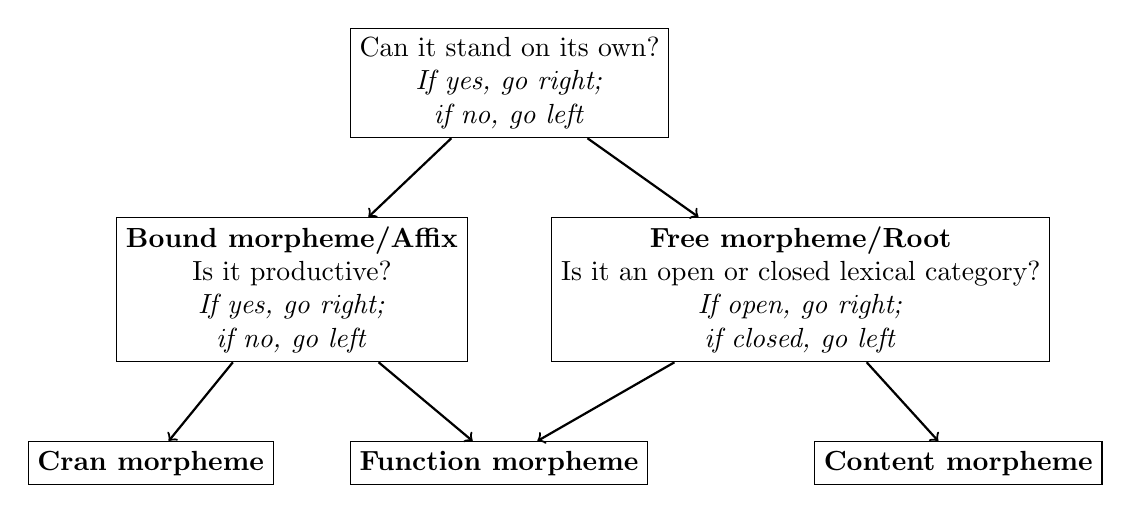
\begin{tikzpicture}
  \node (standing) [process]                                         {Can it stand on its own?\\
                                                                      \emph{If yes, go right;}\\
                                                                      \emph{if no, go left}};
  \node (bound)    [process, below left=1cm and -1.5cm of standing]  {\textbf{Bound morpheme/Affix}\\
                                                                      Is it productive?\\
                                                                      \emph{If yes, go right;}\\
                                                                      \emph{if no, go left}};
  \node (function) [process, below right=1cm and -1.5cm of bound]    {\textbf{Function morpheme}};
  \node (cran)     [process, below left=1cm and -2cm of bound]       {\textbf{Cran morpheme}};
  \node (free)     [process, below right=1cm and -1.5cm of standing] {\textbf{Free morpheme/Root}\\
                                                                      Is it an open or closed lexical category?\\
                                                                      \emph{If open, go right;}\\
                                                                      \emph{if closed, go left}};
  \node (content)  [process, below right=1cm and -3cm of free]       {\textbf{Content morpheme}};
  \draw [arrow] (standing) -- (bound);
  \draw [arrow] (bound)    -- (function);
  \draw [arrow] (bound)    -- (cran);
  \draw [arrow] (standing) -- (free);
  \draw [arrow] (free)     -- (function);
  \draw [arrow] (free)     -- (content);
\end{tikzpicture}

          \end{adjustbox}
        }
        \only<17>{
          \begin{alertblock}{Be careful}
            \begin{itemize}
              \item Only split words up into real morphemes
              \begin{itemize}
                \item \lexi{Catalog} doesn't contain \lexi{cat}
              \end{itemize}
              \item Long words don't automatically have multiple morphemes
              \begin{itemize}
                \item \lexi{Lugubrious} is one morpheme
              \end{itemize}
            \end{itemize}
          \end{alertblock}
        }
      \end{frame}

    \subsection{\subtwofive}
      \begin{frame}{\subtwofive}
        \begin{block}{Try these}
          \textcite{dawson_language_2016}, chapter 4 exercises 2, 3, and 4
        \end{block}
      \end{frame}

    \begin{frame}{References}
      \printbibliography
    \end{frame}
\end{document}
